A finite game with simultaneous moves and chance can be described by a tuple 
$(\cN, \cS = \cD\cup\cC\cup\cZ, \cA, \cT, \Delta_c, u_i, s_0)$.
The player set $\cN = \{ 1, 2, c \}$ contains player labels, where 
$c$ denotes the chance player and by convention a player is denoted $i \in \cN$.
$\cS$ is a set of states, with $\cZ$ denoting the terminal states, $\cD$ the states where players make decisions, 
and $\cC$ the possibly empty set of states where chance events occur. $\cA = \cA_1 \times \cA_2$ is the set of 
joint actions of individual players. We denote $\cA_i(s)$ the actions available to player $i$ in state $s \in \cS$. 
The transition function $\cT : \cS \times \cA_1 \times \cA_2 \mapsto \cS$ defines the successor state given a current 
state and actions for both players. $\Delta_c:\cS \mapsto \Delta(\cS)$ describes a probability distribution over 
possible successor states of the chance event. If node $s$ is not a chance node ($s \in \cD$), $\Delta_c(s)$ assigns $s$ with probability $1$.
The utility functions $u_i : \cZ \mapsto [v_{\min}, v_{\max}] \subseteq \mathbb{R}$ gives the utility of player $i$, with 
$v_{min}$ and $v_{\max}$ denoting the minimum and maximum possible utility respectively. We assume constant-sum 
games: $\forall z \in \cZ, u_1(z) = k - u_2(z)$. 
The game begins in an initial state $s_0$. 

\begin{figure}[t!]
\centering
\begin{tabular}{c|c|c|}
 \multicolumn{1}{c}{~} & \multicolumn{1}{c}{H}  &  \multicolumn{1}{c}{T}\\\cline{2-3}
H &  1  &  0\\\cline{2-3}
T  & 0  &  1\\\cline{2-3}
\end{tabular}
~~~~~~~~~
\begin{tabular}{c|c|c|}
 \multicolumn{1}{c}{~} & \multicolumn{1}{c}{A}  &  \multicolumn{1}{c}{B}\\\cline{2-3}
a &  0  &  1\\\cline{2-3}
b & -1  &  0\\\cline{2-3}
\end{tabular}
\caption{Matrix games of Matching Pennies (left), and one with a pure Nash equilibrium (right). 
Payoffs to the row player are shown. \label{fig:egMatrixGames}}
\end{figure}

A {\it matrix game} is a single step simultaneous move game with action sets $\cA_1$ and $\cA_2$. 
Each entry in the matrix $A_{rc}$ where $(r,c) \in A_1 \times A_2$ corresponds to a payoff (to player 1) if row $r$ is 
chosen by player 1 and column $c$ by player 2. 
For example, in Matching Pennies in the left side of Figure~\ref{fig:egMatrixGames}, each player has two actions (heads or tails). 
The row player receives a payoff of 1 
if both players choose the same action and 0 if they do not match. 
Two-player simultaneous move games are sometimes called {\it stacked matrix games} because at every state 
$s$ there is a joint action set $\cA_1(s) \times \cA_2(s)$ that either leads to a terminal state or (possibly after a 
chance transition) to a subgame which is itself another stacked matrix game. 
In the matrix game on the right of Figure~\ref{fig:egMatrixGames}, $b$ and $B$ are strictly dominated, leaving $(a,A)$ as a 
pure and only Nash equilibrium (NE) strategy.

A {\it behavioral strategy} for player $i$ is a mapping from states $s \in \cS$
to a probability distribution over the actions $\cA_i(s)$, denoted $\sigma_i(s)$. 
Given a profile $\sigma = (\sigma_1, \sigma_2)$, define the probability of reaching a terminal state $z$ under $\sigma$ as 
$\pi^\sigma(z) = \pi_1(z) \pi_2(z) \pi_c(z)$, where each $\pi_i(z)$ is a product of probabilities of the actions taken 
by player $i$ along the path to $z$ ($c$ being chance's probabilities). Define $\Sigma_i$ to be the set of behavioral 
strategies for player $i$. A Nash equilibrium profile in this case is a pair of behavioral strategies optimizing
\begin{equation}\label{eq:ne}
V^* = \max_{\sigma_1 \in \Sigma_1} \min_{\sigma_2 \in \Sigma_2} \bE_{z \sim \sigma}[u_1(z)]
   = \max_{\sigma_1 \in \Sigma_1} \min_{\sigma_2 \in \Sigma_2} \sum_{z \in Z} \pi^\sigma(z) u_1(z).
\end{equation}
In other words, none of the players can improve their utility by deviating unilaterally. 
For example, the Matching Pennies matrix game has a single state and the only equilibrium strategy is to mix equally between 
both actions, \ie play with a {\it mixed strategy} (distribution) of $(0.5, 0.5)$ giving an expected payoff of $V^* = 0.5$.
Note that using a randomized (often called mixed) strategy is necessary in this game.
Any deterministic strategy of one mplayer can be exploited by the opponent. 
For the same reason, randomized strategies are often necessary also in the multi-stage simultaneous move games. 
If the strategies also optimize Equation \ref{eq:ne} in each subgame starting in an arbitrary state, the equilibrium strategy 
is termed subgame perfect.

\begin{figure}[t!]
\centering
\begin{subfigure}{12cm}
\centering
\includegraphics[width=8.0cm]{figures/tree}\\
%\includegraphics[width=10.0cm]{figures/goof3}\\
\end{subfigure}%\\
\caption{An example of a two-player simultaneous game without chance nodes which has Matching Pennies as a subgame. %, and a portion of 3-card Goofspiel including chance nodes (bottom).
The dark squares are terminal states. The values shown are optimal values that could be obtained by backward induction.\\
%bbosansky: if that's ok, I have removed the goofspiel figure since I do not think it is specifically referenced anywhere and we do not need to figures. Plus, since we do not specifically experiment with games with chance nodes, it is better not to include the figure :)
\label{fig:example}}
\end{figure}
In two-player constant sum games a (subgame perfect) Nash equilibrium strategy is often considered to be optimal. It guarantees 
the payoff of at least $V^*$ against any opponent. Any non-equilibrium strategy has its nemesis, which makes it win less 
than $V^*$ in expectation. Moreover, subgame perfect Nash equilibrium strategy can earn more than $V^*$ against weak opponents. After the 
opponent makes a sub-optimal move, the strategy will never allow it to gain the loss back.
The value $V^*$ is known as the minimax-optimal value of the game
and is the same for every equilibrium profile by von Neumann's minimax theorem.

\begin{figure}
\begin{center}
\begin{tabular}{ccc}
\includegraphics[scale=1.3]{figures/rps-nfg} & ~~~~~ & 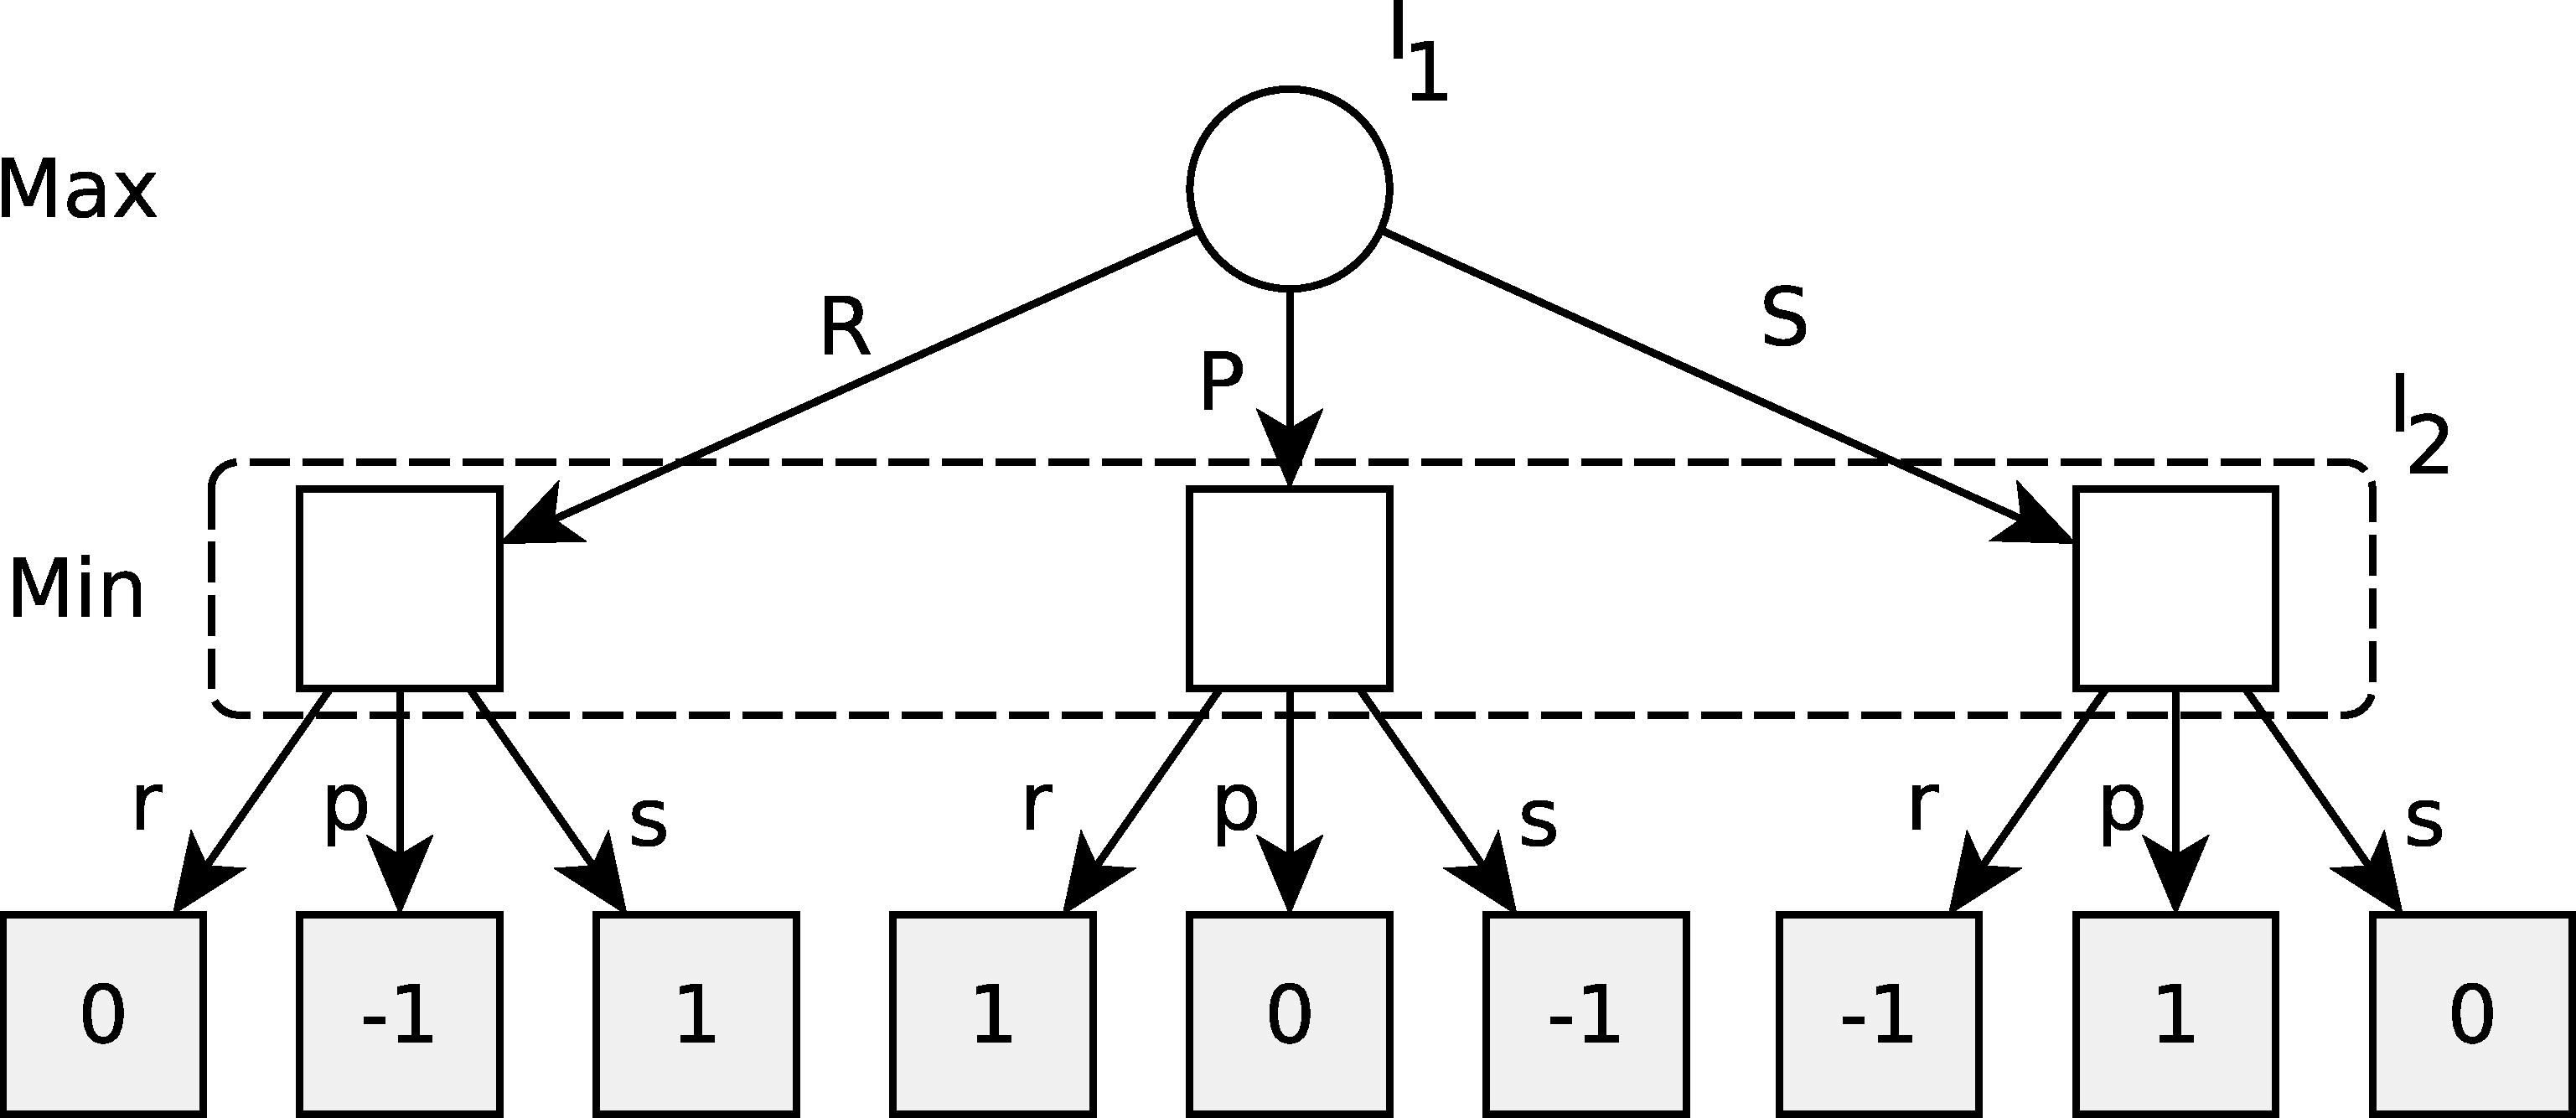
\includegraphics[width=0.6\textwidth]{figures/rps-new} \\
\end{tabular}
\end{center}
\caption{The matrix game of Rock, Paper, Scissors (left) and its equivalent extensive-form game representation (right). The extensive 
game has four states, two information sets ($I_1$ and $I_2$), 
and nine terminal histories: $\{ Rr, Rp, Rs, Pr, Pp, Ps, Sr, Sp, Ss \}$. \label{fig:rps-equiv}}
\end{figure}


A two-player simultaneous move game is a specific type of two-player imperfect information extensive-form game. 
In imperfect information\footnote{In this paper, we use the term {\it imperfect information} to refer to games that have situations 
where one player knows something that some of the other players do not know. However, every player knows which game they are playing, 
the distribution of chance event outcomes, and every player's utility function. This is in contrast to 
{\it imcomplete information} games in which players may also not know (or be fully certain of) the utility functions of their opponents 
or precisely how nature affects the game.} 
games, states are grouped into {\it information sets}: two states $s, s' \in I$ if the player 
to act at $I$ cannot distinguish which of these states the game is currently in. Any simultaneous move game can be modeled 
using information sets to represent a half-completed transition, \ie $\cT(s, a_1, ?)$ or $\cT(s, ?, a_2)$. 
For example, the matrix game of Rock, Paper, Scissors can be thought of as a two-step process where the first player commits
to a choice, writing it on a face-down piece of paper, and then second player responds. Figure~\ref{fig:rps-equiv} shows this
transformation, which can generally be applied to every state in a simultaneous move game by placing the root of subgame following 
both players' decisions, or a successor chance node outcome. 
Therefore, algorithms intended for two-player zero-sum imperfect information games may also be applied to the 
simultaneous move game's equivalent extensive form. 

The model described here is equivalent to two-player finite-horizon Markov Games with chance 
events. An example of such game is depicted in Figure~\ref{fig:example} (more examples can be found in \cite[Chapter 5]{Saffidine2013thesis}).

